%%%%%%%%%%%%%%%%%%%%%%%%%%%%%%%%%%%%%%%%%%%%%%%%%%%%%%%%%%%%%%%%%%%%%%
%%                     Uncertain Process
%%%%%%%%%%%%%%%%%%%%%%%%%%%%%%%%%%%%%%%%%%%%%%%%%%%%%%%%%%%%%%%%%%%%%%
%\color{blue}
\subsection{Glyph: \glyph{Uncertain process}}\label{sec:uncertain}

Uncertain processes are processes that may not exist. A single \glyph{uncertain process} can represent any number of actual processes. \glyph{Uncertain process} would be used to represent hypothesis, reactions which existence is supported by weak evidence etc. An \glyph{uncertain process} is represented by a \glyph{process} which square box contains a question mark.

\begin{figure}[H]
  \centering
  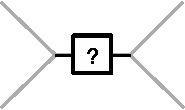
\includegraphics[scale = 0.5]{images/uncertain}
  \caption{The \PD glyph for an \glyph{uncertain process}.}
  \label{fig:uncertain}
\end{figure}

